\section{Service Mesh}

\subsection{Microservice Principles}
The modern architecture of microservices focuses on the following aspects of operation. 
\begin{enumerate}
    \item Deployment Independence
    \item Oranized by business capability
    \item Products not Projects
    \item API Focused
    \item Smart endpoints and dumb pipes
    \item Decentralized governance
    \item Decentralized data management
    \item Infrastructure Automation (IaC)
    \item Design for failure
    \item Evolutionary design
\end{enumerate}

\begin{figure}[h]
    \centering
    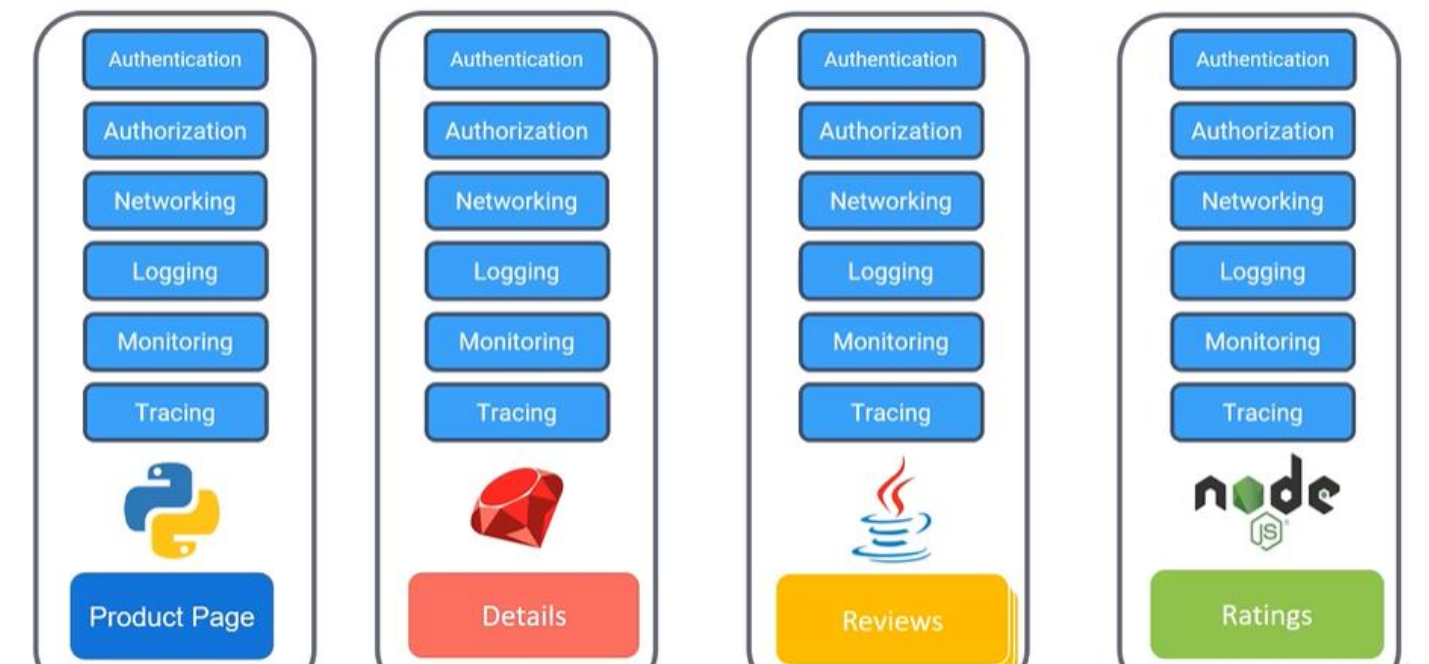
\includegraphics[width=10cm]{servicemesh-traditional}
    \caption{Traditional Service Architecture}
\end{figure}

\subsection{Service Mesh}

A service mesh is a dedicated and configurable infrastructure layer that handles the communication between services without having to change the code in a microservice architecture. 

Instead of every service implementing important functionality themselves, a proxy is deployed to intercept network traffic to each container inside a pod.

\begin{figure}[h]
    \centering
    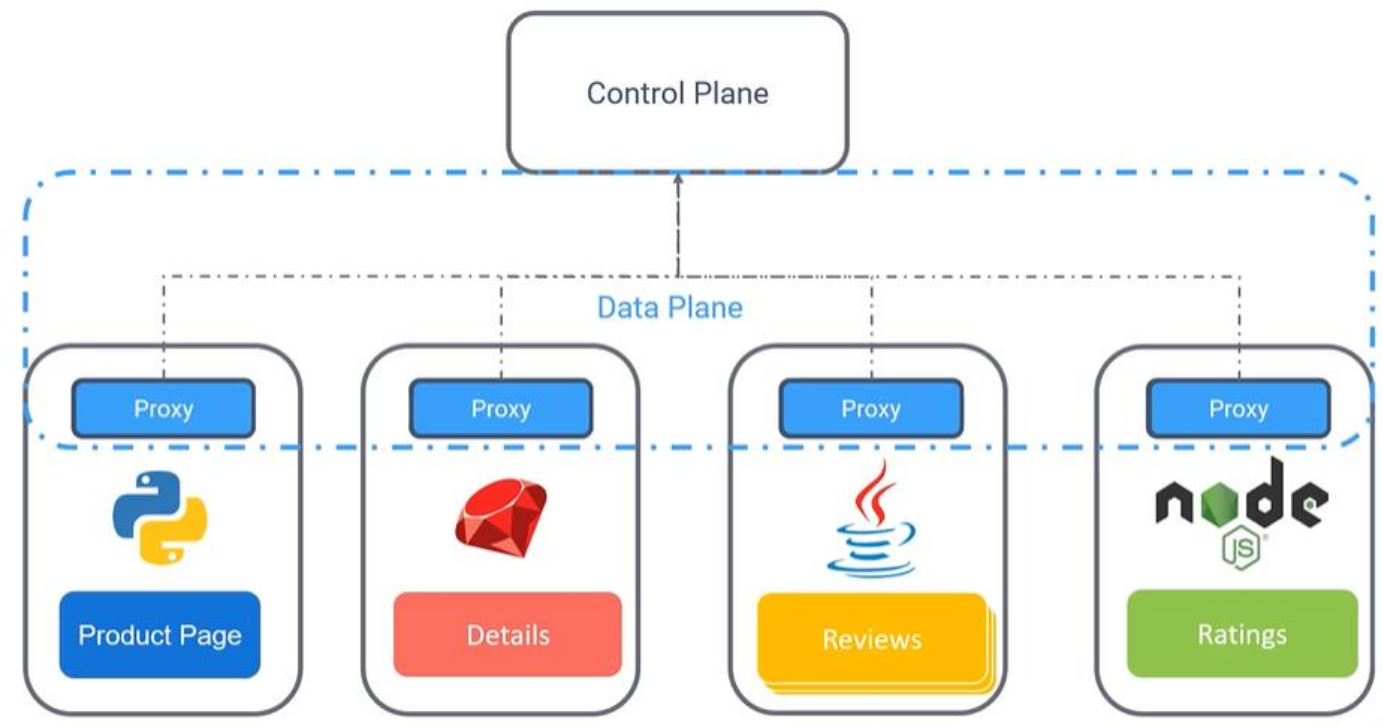
\includegraphics[width=10cm]{servicemesh-new-architecture}
    \caption{Service Mesh Architecture}
\end{figure}

Service Mesh is responsible for Traffic Management, Security, Observability and Service Discovery inside each microservice.
This is done by embedding capabilities via sidecar containers directly into kubernetes pods.

\subsection{The Istio Approach}
\renewcommand{\arraystretch}{1.5}
\begin{center}
    \begin{tabular}{l|l}
        Grafana & Visualization of metrics collected by Prometheus \\
        \hline
        Istio Ingress Gateway & Envoy Proxy which serves as an entry point for the service mesh \\
        \hline
        Istiod & Backbone of the Istio control plane, configures sidecar proxies \\
        \hline
        Jaeger & Provides tracing functionality for traffic inside the service mesh \\
        \hline
        Kiali & Istio dashboard \\ 
        \hline
        Prometheus & Collects monitoring information from sidecar proxies \\
    \end{tabular}
\end{center}

\subsection{Canary Deployment}
Canary deployments are used to test a new version of a microservice in production. To do so, the new version gets deployed, but only a small percentage of traffic gets sent to it. 
If no problems occur and no customers complain, the traffic rate to the new version gets increased. 

\subsection{Virtual Services}
Inside a VirtualService configuration file, a set of traffic routing rules can be defined that should be applied when a host is addressed. 
Each routing rule defines matching criteria for traffic of a specific protocol.

If traffic is matched, it is sent to a named destination service or a specific subset / version of it. This can be used for load balancing and different deployment strategies.

\subsection{Jaeger Spans and Traces}
A trace represents a single request through the service mesh which gets handled by the services. Each unit of work inside a trace is called a span. Spans can be requests to other services, for example.